\section{Grundlagen und Stand der Wissenschaft}
\todo[inline, color=green]{Vera}
Im folgenden werden die Grundlagen und der Stand-der-Wissenschaft von allen Teilbereichen des \text{MArC} Systems erläutert. Es werden Veröffentlichungen von ähnlichen Architektur VR Anwendungen, haptischen Interaktionsmethoden sowie Handtracking Methoden erläutert. Fortlaufend wird auf die Grundlagen der Netzwerktechnologie und den bekanntesten Bedienkonzepten in VR- Umgebungen eingegangen. Zuletzt werden die wichtigsten Methoden zum Marker Verfolgung zusammengefasst.
\subsection{Architektur von Virtual-Reality-Anwendungen}\label{sec:ArchitekturAnwendungen}\todo[inline, color=green]{Lukas}
Bei der Entwicklung von Virtual Reality (VR) Anwendungen gibt es zwei entscheidende Unterschiede im Vergleich zu normalen Software-Anwendungen~\cite{bryson1995approaches}:
\begin{itemize}
	\item die virtuelle Umgebung und das damit verbundene Interface sollten auf die vorliegende Aufgabe zugeschnitten werden und
	\item spezielle Anforderungen an die Performanz der Anwendung müssen erfüllt sein, damit die virtuelle Realität erfolgreich präsentiert werden kann.
\end{itemize}

Als grundsätzlich unterschiedliche Architekturen bei der Entwicklung von VR-An\-wen\-dung\-en kann nach Hardware-Plattformen unterschieden werden:
\begin{description}
	\item[Desktop-VR-Applikationen:] hierbei handelt es sich um die leistungsstärksten VR-Applikationen, die potente Computer-Hardware häufig mit Head-Mounted-Displays wie etwa Oculus Rift oder HTC Vive verwenden.
	\item[Mobile-VR-Applikationen:] mobile Anwendungen vereinen häufig (jedoch nicht immer) alle notwendige Hardware in einem Gerät, wie etwa einem Smartphone oder Tablet-Computer.\\ Beispiele für mobile VR-Anwendungen sind Samsung GearVR~\cite{website:gearVRpressRelease} und Google Cardboard~\cite{website:googleCardboard}. Im Falle von Samsung GearVR und Google Cardboard wird zusätzlich eine Haltevorrichtung für das verwendete Gerät eingesetzt, die bei GearVR auch als Controller fungiert und durch ein integriertes Linsensystem das Sichtfeld des Benutzers erhöht.
	\item[Web-VR-Applikationen:] Anwendungen für das Web wie etwa WebVR~\cite{website:webVR} erlauben den Zugriff auf Virtual-Reality-Geräte wie Head-Mounted-Displays durch einen Browser. Auf diese Weise können Web-Inhalte mit VR-Hardware konsumiert werden.
\end{description}

Die Entscheidung, für das vorliegende Projekt auf eine Desktop-VR-Anwendung zu setzen, wurde getroffen, weil mobile und Web-VR-Applikationen die folgenden, vom Projektteam als unverzichtbar eingestuften, Voraussetzungen nicht erfüllen konnten.
\begin{itemize}
	\item Es sollte möglich sein, die in \ref{sec:HandtrackingAnwendungen} beschriebenen Handtracking Interaktionsmethoden für die Verwendung von haptischen Würfel-Markern zu verwenden.
	\item Außerdem sollte die verwendete Architektur ein zuverlässiges Echtzeit-Tracking mit geringer Latenz von mindestens einem Dutzend Markern erlauben, wie es in \ref{sec:MarkerTracking} beschrieben wird.
	\item Und schließlich sollte \emph{MArC} die Basis bereitstellen, um später auch mit mehreren Benutzern verwendet werden zu können.
\end{itemize}

\subsection{Haptische Interaktionsmethoden in VR Umgebungen}\label{sec:HaptikAnwendungen}\todo[inline, color=green]{Laura}
Um das Eintauchen in die virtuelle Welt zu erleichtern, kann es bei manchen VR-Anwendungen sinnvoll sein, dem Benutzer eine Form von haptischem Feedback zu geben. Die meisten Systeme haben ihren Ansatzpunkt an den Fingern, oder genauer gesagt an den Fingerspitzen. Es gibt aber auch Systeme die mehrere Parts des Körpers oder sogar den ganzen Körper mit einbeziehen.\\
Man unterscheidet zwischen \textit{Active Feedback Devices} und \textit{Passive Feedback Devices}. Während die aktive Variante dynamisch veränderliche Kräfte erzeugt, die dem Benutzer entgegenwirken, werden die passiven Varianten immer nur durch den Benutzer selber bewegt \cite{Haptic}.\\
Um eine genauere Unterteilung vorzunehmen, kann man die verschiedenen Systeme zudem nach den einzelnen haptischen Wahrnehmungen unterteilen. Eine mögliche Aufteilung ist im Folgenden zu sehen.

\begin{description}
	\item[Force Feedback Systeme:] Ausübung eines Kraftvektors auf eine Körperstelle des Benutzers, um seine Bewegung zu erschweren oder aktiv eine Bewegung zu erzwingen. %Ein Beispiel hierfür ist das Exoskelett für die Hand von \textit{Dexta Robotics} \cite{Gu:2016:DIL:2858036.2858487}.
	\item[Tactile Feedback Systeme:] Stimulation der Berührungsempfindung der Haut. Im Allgemeinen wird ein variabler Druck auf eine Hautstelle ausgeübt, welcher nicht direkt von der Bewegung des Körperteils abhängig ist.
	\item[Greifen:] Kann als Kombination der beiden vorangegangen Ansätze angesehen werden. Befindet sich ein virtueller Gegenstand in der Hand so soll hierbei verhindert werden können, dass der Benutzer seine Hand schließt. 
	\item[Proprioceptive Feedback Systeme:] Im Gegensatz zu den \textit{Tactile Feedback Systems} spürt der Anwender nicht über seine Haut, sondern über Gelenke bzw. Muskeln. 
\end{description}

Bei den oben aufgelisteten Formen von haptischer Interaktion wird davon ausgegangen, dass der Gegenstand um den es geht rein virtueller Natur ist. Eine Besonderheit an \textit{MaRC} ist, dass es sich um reale Objekte (siehe Kapitel \ref{sec:WürfelMarker}) handelt, an der Position virtuelle Objekte gerendert werden können. In diesem \textit{Mixed Reality}--System hat der Benutzer also einen realen haptischen Eindruck. Der reale Würfel dient somit als Anfasser und bietet die Möglichkeit das virtuelle Objekt, was durchaus kleiner oder größer als sein reales Pendant sein kann, zu transformieren. 

%In manchen Fällen kann es schwierig sein eine eindeutige Zuordnung des Systems zu einer der Kategorien zu finden.


\subsection{Handtracking Interaktionsmethoden}\label{sec:HandtrackingAnwendungen}\todo[inline, color = green]{Paul}
Handtracking ist mittels verschiedener Trackingsysteme möglich. Alle Systeme haben hierbei ihre Vor- und Nachteile. \\
Beispielsweise ist es möglich, die Bewegungen der Hand mittels eines Datenhandschuhs zu erfassen. Dies ist ein mit Sensoren ausgestatteter Handschuh, den der Nutzer an den Händen trägt. Eine Möglichkeit die Fingerbewegung mit einem Datenhandschuh zu erfassen sind Biegesensoren. Hierbei handelt es sich je nach Bauart um Glasfasern, die an den Fingern entlang laufen. Wird ein Finger gebogen, wird ein Licht welches durch die gebogene Glasfaser läuft, leicht abgeschwächt. Hierdurch ist eine Biegung erkennbar. Dieses System ist ebenfalls mittels gefärbter Flüssigkeit innerhalb kleiner Röhrchen möglich. Auch hier werden bei Bewegung weniger Partikel durchgelassen.\\
Eine weitere Möglichkeit ist das Exosklett. Hierbei wird eine Mechanik an dem Handschuh angebracht, mittels welcher Bewegungen auf Sensoren übertragen werden. Datenhandschuhe sind für den Nutzer einschränkend und aus Hygienischen Gründen nicht die Beste Wahl zum Handtracking.\\
Eine bessere Möglichkeit ist das optische Tracking der Hande. Systeme wie der \textit{Leap Motion Controller} erfassen mit Kameras die Shilouette der Hände und rechnen aus den stereoskopischen Bildinformationen die Winkel und Positionen der verschiednen Fingerglieder aus.\\
Dieses System ist einfach zu benutzen, sobald der Nutzer seine Hand in den getrackten Bereich hält, werden diese erkannt.\\
Typisch für optische Systeme ist jedoch das Problem der Verdeckung. Wird die Hand aus einer bestimmten Richtung durch Kameras gefilmt, kann es passieren, dass einige Finger andere überdecken. Teilweise kann dann nicht exakt unterschieden werden, welches Fingerlied zu welchem Finger oder Teil der Hand gehört. Dies wirkt sich bei der Benutzung in einem "hüpfenden" Verhalten oder unmenschlich verrenkter Finger aus.


\subsection{ISO/OSI-7-Schichtenmodell}\label{sec:Netzwerk}\todo[inline, color=green]{Laura}
Um die Kommunikation zwischen unterschiedlichsten technischen Systemen zu ermöglichen und zu vereinheitlichen dient das \textit{ISO/OSI-7-Schichtenmodell} \cite{ITU}, welches in Tabelle~\ref{tab:Schichtenmodell} schematisch dargestellt ist. Um die Weiterentwicklung von Kommunikationsmodellen möglichst barrierefrei zu gestalten, sind in dem Modell sieben aufeinanderfolgende Schichten definiert worden, die für einen klar eingegrenzten Teilbereich der Kommunikation zuständig sind. Die Netzprotokolle, die in einer Schicht zum Einsatz kommen, müssen einheitliche Schnittstellen aufweisen, um einen reibungslosen Austausch zu gewährleisten. Entsprechende Beispiele sind der rechten Spalte von Tabelle~\ref{tab:Schichtenmodell} zu entnehmen.\\

\begin{table}
	\centering
	\renewcommand{\arraystretch}{1.4}
	\begin{tabular}{|c|c|c|}
		\hline
		\Absatzbox{}
		\textbf{Nr.} & \textbf{Schicht}&\textbf{Beispiel}\\
		\hline
		7 & Anwendung &  HTTP, SMTP, FTP, DNS\\
		\hline
		6 & Darstellung & HTTP, SMTP, FTP, NNTP, NetBIOS\\
		\hline
		5 & Sitzung& HTTP, SMTP, FTP, NNTP, NetBIOS, TFTP\\
		\hline
		4 & Transport & TCP, UDP, SPX, NetBEUI\\
		\hline
		3 & Vermittlung& IP IPX\\
		\hline
		2 & Sicherung & Ethernet, ATM, FDDI, TR\\
		\hline
		1 & Bitübertragung & Manchester, 10B5T, Trellis\\
		\hline
	\end{tabular}
	\caption{ISO-/OSI-7-Schichtenmodell}
	\label{tab:Schichtenmodell}
\end{table}

Während die Schichten 1--4 als transportorientierte Schichten einzustufen sind, können die verbleibenden Schichten 5--7 als anwendungsorientiert angesehen werden. Da der Austausch von Daten für die Umsetzung von \textit{MaRC} im Vordergrund steht, wird im Folgenden besonders auf die vierte Schicht eingegangen. Dabei werden die beiden Übertragungsprotokolle \textit{Transmission Control Protocol} (TCP) und \textit{User Datagram Protocol} (UDP) vorgestellt. Auf die Aufführung weiterer Übertragungsprotokolle wird bewusst verzichtet.\\
Die Transportschicht stellt eine logische Ende-zu-Ende-Verbindungen dar und dient als Bindeglied zwischen den transportorientierten und anwendungsorientierten Schichten \cite{ITU}.

\begin{description}
\item[TCP:] Dieses Transportprotokoll ist verbindungsorientiert und paketvermittelt. Genaue Details können in dem Standard RFC 793 \citep{rfc793} von 1981 in Erfahrung gebracht werden.

\item[UDP:] Dieses Transportprotokoll wurde aus der Notwendigkeit heraus entwickelt, für die Übertragung von Sprache auf ein, im Gegensatz zur TCP, simpleres Protokoll zurückgreifen zu können. Genaue Details können in dem Standard RFC 768 \citep{rfc768} von 1981 in Erfahrung gebracht werden.
\end{description}

Ein wichtiger Unterschied zwischen den beiden Transportprotokollen ist, dass die Übertragung per TCP im Vergleich zu UDP sicherstellt, dass gesendete Daten korrekt übertragen und empfangen werden. \textcolor{red}{QUELLE??} Dies geschieht dadurch, dass in einem TCP-Socket-Netzwerk Fehlererkennungs- und Korrekturmechanismen enthalten sind, die fehlerhafte Übertragungen der darunterliegenden Internet Protocol (IP) Schicht ausgleichen, also entweder korrigieren oder dafür sorgen, dass fehlerhafte Daten erneut übertragen werden.

\subsection{Bedienkonzepte in VR-Umgebungen}\label{sec:MenüAnwendungen}\todo[inline, color=green]{Lukas}
Die Bedienung eines Systems~--~vor allem Dateneingabe und Objektmanipulation~--~in einer Virtual Reality (VR) Umgebung unterscheidet sich stark von der konventionellen Bedienung mit Maus und Tastatur \cite{chu1997multi}. Das Hauptziel einer VR-Umgebung ist Immersion, also das "`Eintauchen"' des Benutzers in die virtuelle Welt. Ein Teil zur Erreichung dieses Ziels sind Methoden, mit denen der Benutzer mit der virtuellen Welt~--~möglichst intuitiv~--~interagieren kann.

Nach~\cite{sherman2002understanding} gibt es vier unterschiedliche Manipulationsmethoden für VR-An\-wen\-dung\-en:
\begin{description}
	\item[Direct User Control:] Der Benutzer interagiert mit Objekten in der virtuellen Welt so, wie dieser es auch in der realen Welt tun würde. Ein Beispiel hierfür ist eine Geste wie das Schließen der Hand zu einer Faust, um einen Gegenstand in der virtuellen Welt "`anzufassen"', sodass dieses Objekt anschließend der Bewegung der Hand folgt.
	\item[Physical Control:] Manipulationen in der virtuellen Welt geschehen durch die Interaktion des Benutzers mit einem realen Gegenstand. Ein solcher Gegenstand kann beispielsweise ein Lenkrad oder ein Joystick sein.
	\item[Virtual Controls:] Bei \emph{Virtual Controls} handelt es sich nicht direkt um eine Manipulationsmethode, viel mehr beschreibt der Begriff die in der virtuellen Welt vorhandenen Interaktionsmodule, wie etwa Buttons, die gedrückt werden können. Um tatsächlich zu interagieren muss der Benutzer eine der drei anderen Manipulationsmethoden verwenden.
	\item[Agent Controls:] Der Benutzer interagiert mit der virtuellen Welt über einen "`intelligenten Mittelsmann"'. Dieser Mittelsmann kann eine Person oder ein vom Computer kontrolliertes Wesen sein.
\end{description}
In den Abschnitten~\ref{sec:kontextMenu}, \ref{sec:markerHandles} und \ref{sec:TableMenü} wird auf die in \emph{MArC} verwendeten Interaktions- und Manipulationsmethoden eingegangen.

\subsection{Marker Verfolgung} \label{sec:MarkerTracking}\todo[inline, color=green]{Vera}
In einer VR oder AR Umgebung ist zur interaktiven Positionierung eines 3D Objektes die präzise Bestimmung der Orientierung und Position im 3D-Zielraum notwendig. Zur Lösung dieses Problems muss zunächst ein physisches Objekt in der realen Welt erkannt, zugeordnet und verfolgt werden. Demzufolge ist es notwendig dieses physische Objekt mit einer Videokamera aufzunehmen. In den resultierenden Bildsequenzen werden die physischen Objekte anhand von festgelegten Merkmalen erkannt. Diese Merkmale können sowohl natürlicher Art sein oder in Form von künstlich erstellten Codes festgelegt sein. Ein Objekttracking mit natürlichen Merkmalen wird in der Literatur auch als \textit{Markerless Tracking} bezeichnet, während die Verwendung von Codes, beziehungsweise Bildmarken, als \textit{Markerbased Tracking} bekannt ist.

Natürliche Merkmale zur Identifizierung der Objekte sind Textureigenschaften, Kanteninformationen oder sogenannte Keypoints. Eine der robustesten und simpelsten Methoden ist die Verwendung von Keypoints \cite{article:MarkerLessBarandiaran2010}\cite{article:MarkerLessWagner:}\cite{article:MarkerLessComport}\cite{article:MarkerLessLowe}, die sowohl in der Ausgangs- als auch in der Kamerawelt bekannt beziehungsweise ermittelbar sind. Diese werden mit Hilfe einer Homographie zur Übereinstimmung gebracht. Daraus resultiert die notwendige Transformation zwischen den Welten (siehe Kapitel \ref{sec:calib}). Ein bedeutender Nachteil der Verwendung von Keypoints oder Texturbasierten Verfahren ist, dass sie nur für Objekte mit einem hohen Grad an Texturmerkmalen und großen Gradientenbeträgen geeignet sind. Aus diesem Grund wurden auch Verfahren \cite{article:MarkerLessStrucktHinterstoisser}\cite{article:MarkerLessStrucktDamen}\cite{article:MarkerLessStrucktPark} entwickelt die sich speziell für texturarme Objekte eignen, wie etwa die in \textit{MArC} verwendeten grünen Rechtecken der Würfel Marker (siehe Kapitel \ref{sec:WürfelMarker}). Andere Autoren verwenden sehr rechenintensive Kantenerkennungsalgorithmen, wie den \textit{Moving Edges Algorithm} \cite{article:MarkerLessEdgeMarchand}. Eine weitere Weiterentwicklung der Kantenbasierten Methoden ist das Modelbased Tracking bei dem die detektierten Kanten eines möglichen Kandidaten mit den 3D-Kantenmodellen des zu verfolgenden Objektes abgeglichen wird \cite{article:MarkerLessModellVacchetti}\cite{article:MarkerLessEdgeAlvarez}\cite{article:MarkerLessEdgeWu}\cite{article:MarkerLessBlasko}.

Im Gegensatz zu dem \textit{Markerbased Tracking} benötigt das \textit{Markerless Tracking} keine Veränderung oder Anpassung der realen Welt. Doch die Parameter, welche den Tracking-Algorithmus beeinflussen, können nicht ohne Weiteres kontrolliert werden \cite{article:MarkerLessBarandiaran2010}. Dennoch ist das \textit{Markerless Tracking} von Objekten sehr rechenaufwändig und eine eindeutige Zuordnung beziehungsweise Identifikation von ähnlichen oder gleichförmigen Objekten, wie zum Beispiel den Würfel Marker, ist sehr aufwändig und nahezu unmöglich. Aus diesem Grund ist es für ein System wie \textit{MArC} zum derzeitigem Zeitpunkt sinnvoller die Würfel Marker mit codebasierten Mustern zu erweitern, die auch nach längerer Verdeckung eine eindeutige Zuordnung von Würfel Marker ermöglichen. In Abbildung \ref{fig:BinMarker} sind vielfältige Beispiele von binären Codes zu sehen, die zum Marker Tracking verwendet werden. Für \textit{MArC} sind vor allem rechteckige binäre Muster vorteilhaft, da aus dem äußeren vier Ecken auch die Orientierung des Würfel Markers im Raum abgeleitet werden kann. Während der Inhalt des Muster zur eindeutigen Identifizierung des Würfels beiträgt. 

Bekannte markerbasierte Verfahren mit rechteckigen binären Mustern sind das bekannte \textit{QR} Verfahren, \textit{ARToolKit}\cite{article:MarkerARTOOL}, \textit{ARToolKit Plus}\cite{article:MarkerARTOOL2}, \textit{ARTag} \cite{article:MarkerARTag}, \textit{BinARyID}\cite{article:MarkerBinAR} und \textit{ArUco}\cite{article:Aruco2014}. Wie in Abbildung \ref{fig:BinMarker} zu sehen ist, sind bis auf \textit{BinARyID} und \textit{ArUco} alle Muster sehr detailreich und komplex. Diese Eigenschaft ist auf die höhere Bitanzahl der Codes zurückzuführen macht die Erkennung in Aufnahmen aus größerem Abstand und möglicher mit Bewegungsunschärfe ungleich schwerer. Es kommt unter diesen Umständen häufiger zu Fehlinterpretationen und Ausfällen. Gerade in einem System wie \textit{MArC} tritt Bewegungsunschärfe sehr häufig aus, da die Würfel Marker regelmäßig bewegt werden. Auch der verhältnismäßig große Abstand der Kamera zu den Würfel Markern lässt die Markermuster im Kamerabild relativ klein werden und somit wirkt sich die Bewegungsunschärfe noch deutlicher auf die feinen Codemuster aus. Darum eigen sich hier vor allem Muster mit geringer Bitanzahl und groben Mustern, wie zum Beispiel \textit{ArUco} Marker mit einer $16$ bit Codierung. Diese Marker Bibliothek ist ein \textit{OpenCV} Modul (siehe Kapitel \ref{sec:OpenCV}), welche alle notwendigen Funktionalitäten und Ressourcen für das Tracking und die Orientierungsbestimmung der physische Objekt enthält. Ein weiterer großer Vorteil dieser Bibliothek ist, dass die Bitgröße und maximale Anzahl der Identitäten explizit ausgewählt werden kann.


\begin{figure}[H] 
	\center 
	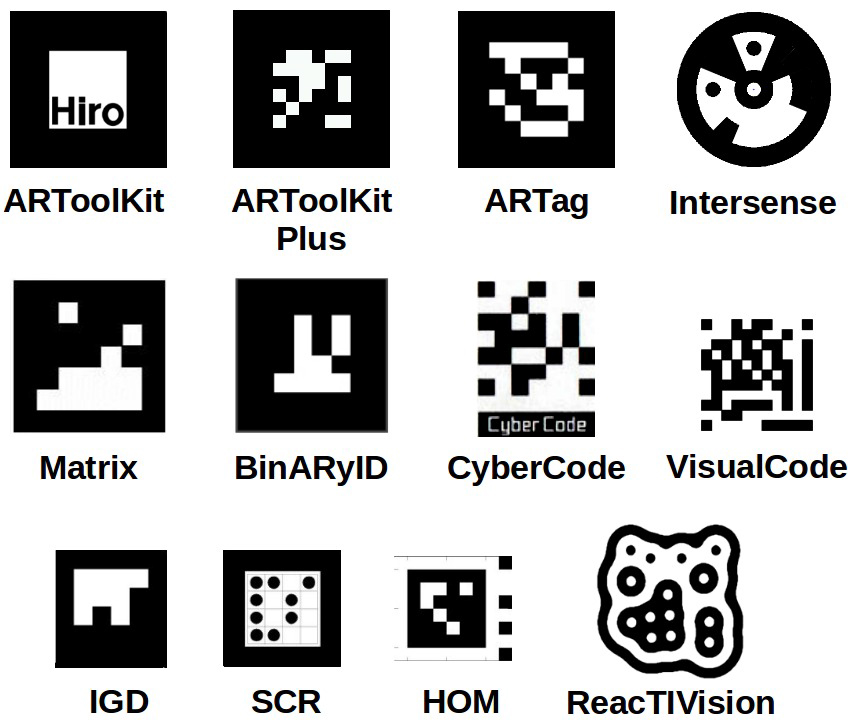
\includegraphics[width=8cm]{Bilder/BinMuster.jpg}			
	\caption{Diverse Binäre Muster die als Code für Markerbasiertes Tracking verwendet werden. Quelle: \cite{article:Aruco2014}}
	\label{fig:BinMarker}
\end{figure}

\newpage